\documentclass[12pt,twoside]{article}

\usepackage{amsmath}
\usepackage[utf8]{inputenc}
\usepackage{template}
\usepackage{lipsum}

\usepackage{apacite}
\bibliographystyle{apacite}

\usepackage{Sweave}
\begin{document}
\Sconcordance{concordance:report.tex:report.Rnw:%
1 10 1 1 0 68 1 1 18 19 1 1 8 15 1 1 17 19 1 1 29 14 0 1 2 1 1 1 22 10 %
1 1 25 10 1 1 9 14 1 1 4 20 0 1 2 13 1}


\begin{titlepage}
\newcommand{\HRule}{\rule{\linewidth}{0.5mm}} 

\center % Center everything on the page

%	TITLE SECTION

\mbox{ }
\vspace{75mm}

%\HRule \\[0.8cm]
{ \Huge \bfseries \color{black}{Analysis of whistler weather data}}\\[0.4cm] 
%\HRule \\[1.5cm]

{\Large
\textsl{Stat 300 Project, Fall 2015}}

\bigskip
{\Large
by Nathan Esau, Ethan Sim, Benjamin Chan}

\vfill

%\vspace{15mm}
%\begin{figure}[!ht]
%\begin{center}
%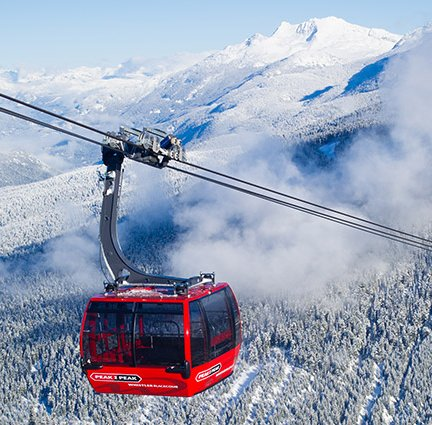
\includegraphics[width=0.9\textwidth]{tp_picture.jpg}
%\end{center}
%\end{figure}

%\vfill
%{\large
%Stat 300 Group Project \\ 
%\medskip
%Fall 2015}

\end{titlepage}

%\thispagestyle{firststyle}
%\noindent
%{\Large \textbf{Analysis of Whistler Weather Data}} 
%
%\medskip\noindent
{%\large \textsl{by Benjamin Chan, Ethan Sim and Nathan Esau}}

\section{Summary}

\subsection{Background}

In this study we analyze daily weather data from Whistler, BC. The variables analyzed were the amount of snow on the ground and the average temperature during each day.

\medskip\noindent
Our study was motivated by trying to answer the following questions:

\begin{enumerate}
\item When is the winter season? When does it start, peak and end?
\item How severe is the winter? How much snow is present at different points in the year? 
\item What trends exist in the data? What odd behaviors have shown up over the past 9 years? 
\end{enumerate}

\subsection{Methods}

\noindent
To answer our questions, we used the following techniques:

\begin{enumerate}
\item Regression, to determine whether there was a trend in the snowfall data
\item Time series techniques, such as average smoothing, to compare different winter seasons
\item Correlation, to determine how different variables were related
\end{enumerate}

\subsection{Results}

We found that the amount of snow has been downward trending at a rate of -- 4.42 cm annually. The estimated start of winter in Whistler was December 3rd and the estimated end of winter was March 26th. The average length of winter was 114 days. A peak amount of snow of 86 cm occurs around February 12th. The average temperature during the winter was -0.98 degrees celsius. The shortest winter was the 2009--2010 season, which started on Nov 14th and ended on February 7th. This winter season also had the lowest peak amount of snow (58 cm). The average temperature and average snowfall during the winter had a correlation of -0.15.

\subsection{Interpretation}

We found that while temperature is very consistent year to year, the amount of snowfall has been showing a downward trend. In particular, the 2009--2010 winter in which Vancouver hosted the Olympics was far less severe, both in the amount of snow and the duration of snowfall, than typical winter seasons. This was shown by comparing the length, average snowfall and peak snow amount of the 2009--2010 winter to other winters.

By averaging different annual time series, we determined what a typical winter season is like in Whistler. In order to do so, we needed to make an assumption about what constitutes the start and end of winter. We classified winter as the period when the average snow on the ground over a week stayed above a given threshold. This contrasts the typical definition of winter as the period from December 21 to March 21.

We also analyzed whether cold winters also tend to have a lot of snow. While these variables do exhibit some negative correlation, we do not have too much evidence that this is necessarily the case.

\section{Introduction}

Whistler Blackcomb is a Canadian resort town in the province of British Columbia, one of the largest ski resorts in North America. Whistler’s economy is highly dependent on the seasonality of snow as the main winter activities offered there are skiing and snowboarding. In July 2003, Whistler was selected to host the alpine skiing events for the 2010 Winter Olympics. However, 2010 was accompanied with an unusually mild winter. The lack of snow made it challenging to run some of the Winter Olympic activities. Given this kind of uncertainty, it would be helpful to have a rough estimate of the when the whistler winter season usually occurs and the peak time of snowfall.

Our weather data was obtained from \url{http://climate.weather.gc.ca/}. Data was recorded at an elevation of 657.80 metres, a longitude of 122$^{\circ}$57'17.400'' W and a latitude of 50$^{\circ}$ 07'44.001'' N over the period 2006 -- 2014. The data set contained the following variables

\begin{itemize}
\item Temperature -- minimum, maximum and mean temperature during each day
\item Snow on the ground 
\item Total precipitation 
\item Wind speed and direction
\end{itemize}

\vspace{-3mm}
\medskip The variables most relevant to answering our questions were the snow on the ground and the temperature. For temperature, we decided to use the mean temperature during each day, as we felt this is the most robust measure. We didn't account for wind, due to the large number of missing and truncated values present, or for precipitation which we felt wasn't related to our question. 

We needed to perform some imputation for our variables. In particular, the snow on the ground during the summer months was not recorded, so we made the assumption that these was no snow on the ground at this point. Also, during the winter period when snow was not recorded we imputed the snow value from the previous day. Similarly, when the temperature was not recorded we imputed the temperature value from the previous day. During the winter, only a small portion of values were missing for these variables ($<5\%$) so this imputation shouldn't have a large impact on our analysis.

Our overall goal was to understand the time series shown in Figure \ref{fig:basicts}. In this figure we have shown the two-week moving average for the amount of snow on the ground and the three-week moving average for the mean temperature.


\begin{figure}[!ht]
\begin{center}
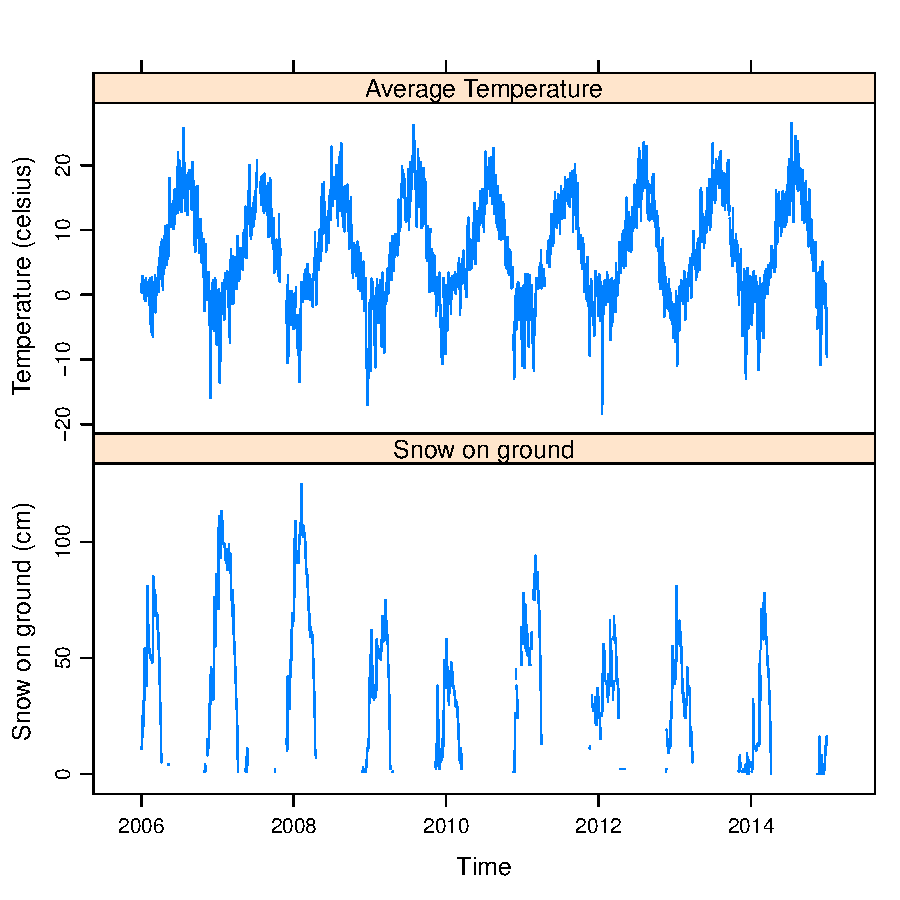
\includegraphics[width=0.8\textwidth]{report-basicts}
\end{center}
\vspace{-5mm}
\caption{Whistler weather data from 2006 -- 2014}
\label{fig:basicts}
\end{figure}

\section{Methods and Results}

Our methods are divided into the following sections. First, we analyze whether a downward trend exists in the amount of snow during our observation period. Second, we average the annual time series and to determine the minimum, maximum and average amount of snow present in Whistler at each day during the year. Finally, we compare the length and severity of each of the winter seasons. For the severity, we look at the average amount of snow and average temperature during the winter, and analyze whether these results are correlated in some way.

\subsection{Trend}

Linear regression was used to fit a trend for snowfall, as shown in Figure \ref{fig:snowtrend}. There is evidence that the amount of snow present in Whistler has been decreasing, as the slope coefficient is highly significant with $p$-value $< 0.001$. However, this downward trend is likely exaggerated due to the fact that we only have 9 years of weather data. 

It is natural to wonder whether this downward trend is a result of rising temperatures (global warming). However, this is little evidence from our data to support this claim. For instance, the average temperatures (shown in Figure \ref{fig:basicts}) don't appear to be increasing  over time. When we tried fitting a trend line to these temperatures, the slope was $0.11$ degrees celsius with $p$-value $>$ 0.01, which makes it difficult to infer causality between the temperature and declining amount of snow.


\begin{figure}[!ht]
\begin{center}
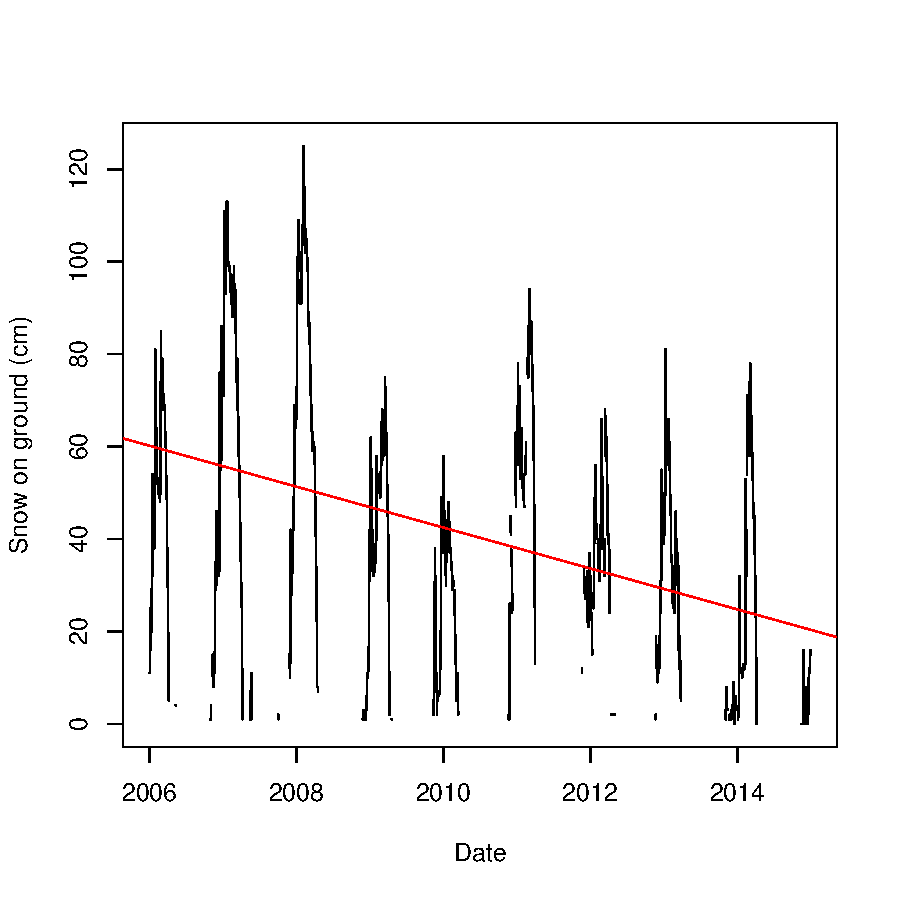
\includegraphics[width=0.7\textwidth]{report-snowtrend}
\end{center}
\vspace{-5mm}
\caption{Snowfall is trending downards at a rate of 4.42 cm per year}
\label{fig:snowtrend}
\end{figure}

\subsection{Average smoothing}

In order to determine how much snow is present at different points in the year, we averaged the 9 annual time series. One complication was that 2008 and 2012 were leap years. We needed the annual time series to be the same length in order to average them, so we removed February 29th of 2008 and 2012 from our data set.

The resulting minimum, maximum and average amount of snow at each day is shown in Figure \ref{fig:averagetsplot}. We have rearranged the dates to show the period July 1 -- June 30 rather than Jan 1 -- Dec 1. Notice that snowfall usually starts at the beginning of November and melts by the end of April. Since the amount of snow was recorded at the base of the mountain, at an elevation of 657.8 metres, it is quite a bit lower than one would expect at the top of the mountain at an elevation of 2,284 metres \cite{WhistlerBlackcomb}.

Figure \ref{fig:averagetsplot} also helps to convey some odd snowfall behavior. From the maximum line, we can see that it is possible to get snow at almost time during the year with the exception of July and August. From the minimum line, we can see that some years do not get any snow until December and have no snow at the mid-way point of April.


\begin{figure}[!ht]
\begin{center}
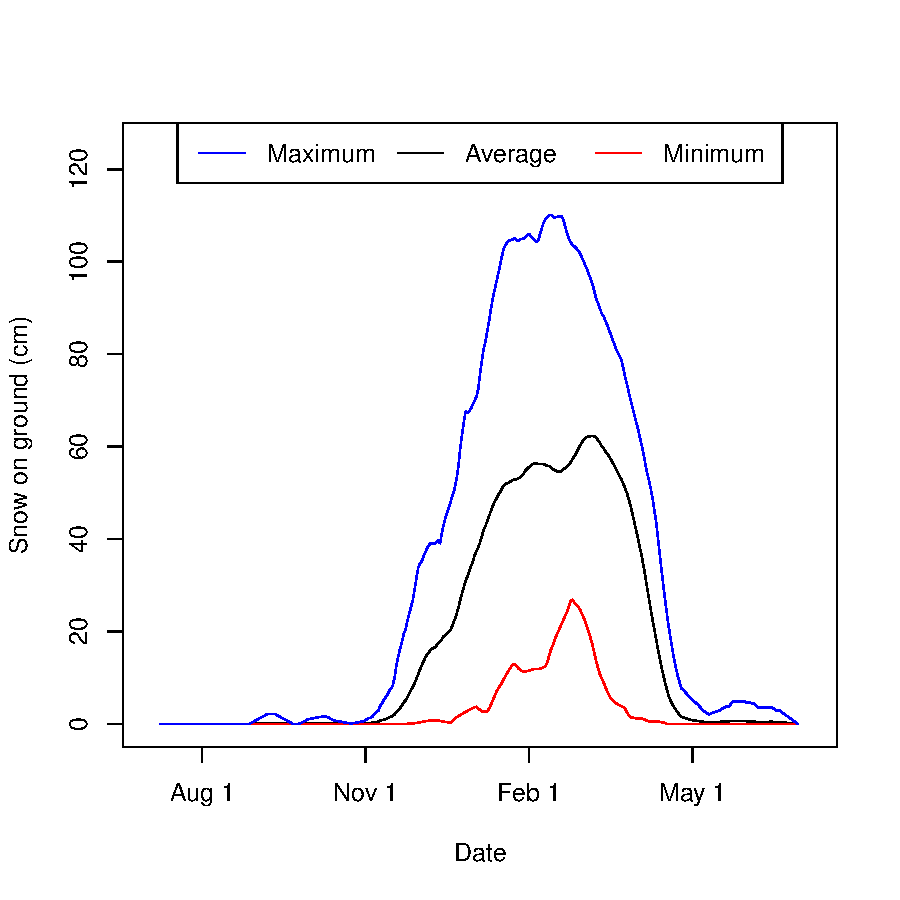
\includegraphics[width=0.7\textwidth]{report-averagetsplot}
\end{center}
\vspace{-8mm}
\caption{Average amount of snow present at each day during the year based on period from 2006 -- 2014}
\label{fig:averagetsplot}
\end{figure}

\subsection{Winter length and severity}

One of goals was to compare the winter season of each of the years. Our criteria for the start of winter was based on a snow threshold as shown in the equation below.
%
\begin{align*}
Winter &= \text{Period when } \text{7 day moving average of} \text{ snow} > \textsl{Threshold} \text{ (cm)}
\end{align*}

\medskip We tried varying the threshold over different values. The length of the winter is shown under a variety of thresholds in Table \ref{tab:robustcheck}. The results are quite similar under the different thresholds, with 2006--2007 and 2007--2008 being the longest winter seasons and 2009--2010 and 2013--2014 being the shortest winter seasons. For the remainder of the analysis we decided to use a threshold of 15 cm.

% latex table generated in R 3.2.2 by xtable 1.8-0 package
% Sat Nov 28 13:04:54 2015
\begin{table}[ht]
\centering
\begin{tabular}{c|rrrrrrrr}
  \hline
Threshold (cm) & 06-07 & 07-08 & 08-09 & 09-10 & 10-11 & 11-12 & 12-13 & 13-14 \\ 
  \hline
10 & 145 & 138 & 108 & 93 & 136 & 143 & 121 & 87 \\ 
  15 & 137 & 135 & 103 & 85 & 128 & 136 & 99 & 87 \\ 
  20 & 134 & 132 & 101 & 78 & 125 & 126 & 94 & 55 \\ 
   \hline
\end{tabular}
\caption{Length of winter under a variety of thresholds} 
\label{tab:robustcheck}
\end{table}
\medskip
The dates associated with each of the winter  seasons are shown in Table \ref{tab:summarytable}. Notice that winter usually starts around December 3 and ends around March 26. However, the 2009--2010 winter ended on February 7, much earlier than the other seasons. This means on February 7, 2010, most of the snow was melted at the base of Whistler mountain, so organizers would have had to bring in extra snow for the Olympics. Also, the 2013--2014 winter had a very late snowfall compared to other seasons, only beginning on January 7.

% latex table generated in R 3.2.2 by xtable 1.8-0 package
% Sat Nov 28 13:04:54 2015
\begin{table}[ht]
\centering
{\small
\begin{tabular}{cccccccc}
  \hline
Winter & Start Date & End Date & Length & Peak Date & Peak Amt & Avg snow & Avg temp. \\ 
  \hline
2006-2007 & Nov 18 & Apr 4 & 137 days & Jan 19 & 113 cm & 72 cm & -0.56 c \\ 
  2007-2008 & Nov 27 & Apr 11 & 135 days & Feb 7 & 125 cm & 73 cm & -1.23 c \\ 
  2008-2009 & Dec 22 & Apr 4 & 103 days & Mar 17 & 75 cm & 48 cm & -1.8 c \\ 
  2009-2010 & Nov 14 & Feb 7 & 85 days & Jan 2 & 58 cm & 30 cm & -1.17 c \\ 
  2010-2011 & Nov 24 & Apr 1 & 128 days & Mar 5 & 94 cm & 59 cm & -1.31 c \\ 
  2011-2012 & Nov 24 & Apr 9 & 136 days & Mar 15 & 68 cm & 38 cm & -0.37 c \\ 
  2012-2013 & Dec 7 & Mar 16 & 99 days & Jan 9 & 81 cm & 41 cm & -1.26 c \\ 
  2013-2014 & Jan 7 & Apr 4 & 87 days & Mar 6 & 78 cm & 37 cm & -0.17 c \\ 
  Average & Dec 3 & Mar 26 & 114 days & Feb 12 & 86 cm & 50 cm & -0.98 c \\ 
   \hline
\end{tabular}
}
\caption{Dates of winter seasons based on a threshold of 15 cm of snow} 
\label{tab:summarytable}
\end{table}
\medskip
The severity of the winter was measured by the average amount of snow present during the winter season. This is shown in Figure \ref{fig:barplots}. We found that the 2009--2010 winter season was less severe than the other winters and only had an average amount of snow of 30 cm present over the period November 14, 2009 to February 7, 2010. We were not able to compute an average for the 2005--2006 winter or 2014--2015 winter since we only analyzed data from 2006--2014. 


The peak amount of snow during a season could also be used as a measure of the severity of the winter. However, the average amount of snow and peak amount of snow (shown in Table \ref{tab:summarytable}) have a correlation of 0.96 so these two metrics are similar.


In Table \ref{tab:summarytable} we also show the average temperature during each winter season. The coldest winter was actually the 2008--2009 winter season and the warmest winter was the 2013--2014 season. There is a correlation of -0.15 between the average snow and temperature during the winter. This means that when temperatures are colder, there tends to be a larger amount of snow. The correlation would slightly change if a different snow threshold were used to identify the winter period. It is possible that other factors, such as wind and precipitation may influence the average amount of snow present. For instance, a strong wind could blow away the snow and change the snow height measured by the weather station. However, this was not part of our analysis.


\begin{figure}[!ht]
\begin{center}
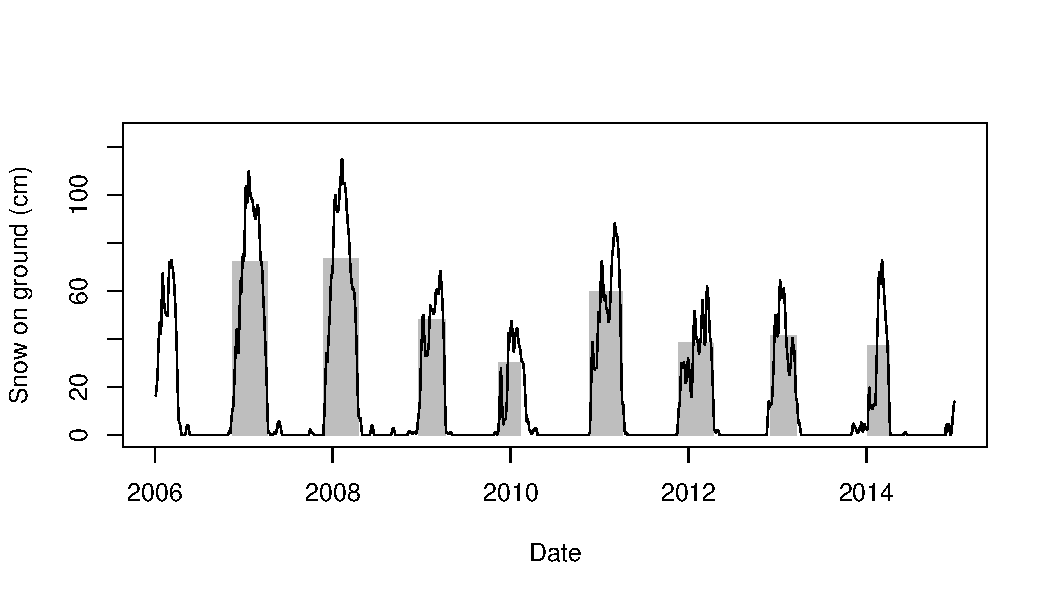
\includegraphics[width=1.0\textwidth]{report-barplots}
\end{center}
\vspace{-8mm}
\caption{Amount of snow on the ground; Lines represent the actual amount of snow at each point in the year; Bars represent the average amount of snow over the winter season}
\label{fig:barplots}
\end{figure}


\section{Conclusion}

We used regression, time series techniques such as average smoothing and correlation to answer our questions. We found that the winter season starts around December 3 and ends around March 26. The maximum snow present is the season is usually around 86 cm and occurs at February 12. The average amount of snow present during the winter is 50 cm. We were not able to fully explain why some winters have more snow then others. Although, this can be partly explained by the temperature (which has a correlation of -0.15 with the snowfall) there are likely other factors, such as wind and precipitation that could affect the amount of snowfall. Answering this kind of question would be an area for future work.

We found that the snowfall has been trending downwards at a rate of 4.42 cm per year based on our data from 2006--2014. However, there is strong uncertainty as to whether future snowfall trends can be accurately predicted. Such an analysis could possibly be done using a seasonal ARIMA model or other techniques. This is also an area for future work.

In summary, we performed exploratory analysis to understand the Whistler weather data over 2006--2014 rather than fitting a predictive model to this data.

\nocite{*}
\bibliography{sources}

\end{document}
